\documentclass[10pt]{article}
\usepackage[a4paper,margin=18mm]{geometry}
\usepackage{amsmath,amssymb,graphicx,hyperref}
\hypersetup{colorlinks=true,urlcolor=blue}
\setlength{\parindent}{0pt}\setlength{\parskip}{6pt}
\begin{document}
\begin{center}\Large A quadratic many-coset interface\\[3pt]
\normalsize Construction and fixed correctness controls, 16 November 2026\\
PCC standing unverified\end{center}
The public-parameter Rust compiler lifts membership in the earlier raw
many-coset base into quadratic equations. Its optional signed elliptic
image emits a nonidentity $[8]P$. It contains no target-sum oracle or
decomposition-cost bound. PCC-20261116-688961. [pcc:unverified]

\begin{center}
\begin{tabular}{lrrrr}
Module & Variables & Equations & Terms & Degree\\\hline
Membership &140&142&423&2\\
With cofactor image &159&161&483&2
\end{tabular}
\end{center}
These count exported representations with different outputs, not attack
running times or a performance comparison.

\begin{center}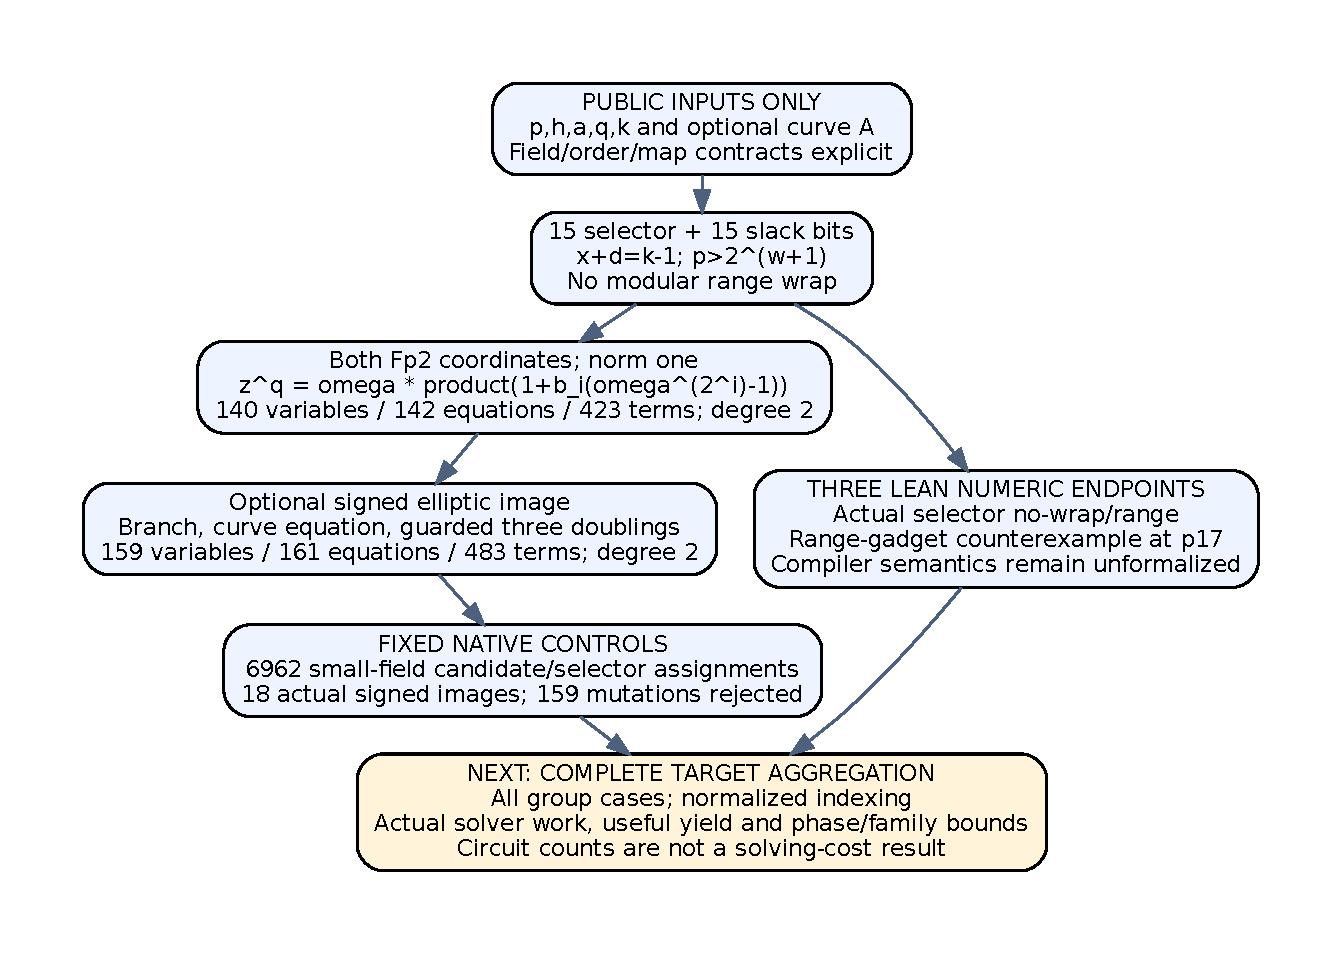
\includegraphics[width=0.98\linewidth,height=118mm,keepaspectratio]{pipeline.pdf}\end{center}

\textbf{External contracts.} Prime field, nonsquare two, norm-one $h$ of
order $aq$, $0<2k<a$, and the actual curve/map hypotheses. The constructor
receives no planted index, point or secret. It does not certify these field,
order or map facts. Actual $a=60824497$, $q=213156431$, $k=20633$,
$p=2^{255}-19$, $A=486662$.

\newpage
\begin{center}\Large Range, image and evidence scope\end{center}
\textbf{Bounded selector.} Fifteen bits encode $x=j-1$ and fifteen slack
bits encode $d$. Boolean equations and $x+d=k-1$, with
$p>2^{w+1}$, encode $0\le x<k$ as integers. Put $\omega=h^q$ and impose
both coordinates of
\[
 z^q=\omega\prod_i\bigl(1+b_i(\omega^{2^i}-1)\bigr),\qquad N(z)=1.
\]
There are 39 Fp2 power gates and 15 selector gates. No $k$-entry table
is used by this circuit. A small lifted graph still has no supplied solving
bound. The earlier primitive-root theorem identifies its membership
predicate under the external instance contracts. [pcc:unverified]

\textbf{Numeric proof scope.} Three new Mathlib-based endpoints cover the
actual cast/no-wrap/range and the range-only example $p=17,x=31,d=3,k=18$:
field equality holds while the integer cap fails. This concerns the generic
range gadget, not a valid full torus instance. The focused gate audits three
named endpoints with no failing or trusted-native exceptions. Boolean
decoding, the compiler and actual Fp2/map bridges remain unformalized.
PCC-20261116-645f28. [pcc:unverified]

\textbf{Signed cofactor image.} A Boolean branch $c$ selects
\[
 u=-A/2+(1-2c)A/(2z_a),\qquad v^2=u^3+Au^2+u.
\]
An inverse witness for $z_a$, a named $u^2$ and three guarded affine
doublings emit $[8](u,v)$. Nonidentity cofactor images have nonzero
doubling denominators; identity images are explicitly outside this retained
interface. Group aggregation must later include equal-point, inverse and
identity intermediates completely. [pcc:unverified]

\textbf{Actual controls.} The small Fp59 fixture has six directly
enumerated members. All 3481 coordinate candidates and both valid selectors
give 6962 canonical gate assignments matching that set. Eighteen fixed signed
Curve25519 images satisfy every equation and match the existing native
curve API's $[8]P$. All 159 single-variable mutations of one actual witness
are rejected, along with malformed values, nonbinary/overflow selectors,
unsafe modulus and a zero doubling denominator. No failed input was omitted.
PCC-20261116-688961. [pcc:unverified]

\textbf{Reproduction.} Native pre-call source/binary digests, full trace,
first witness, compressed complete systems, 38 source/manifest hashes and a
45784-byte post-check archive are retained. Release tests, fmt and strict
Clippy pass. Failed initial Lean/lint attempts are separate. These are local
software/kernel checks, not signed execution or a verified compiler.
No solver, sampling, timing experiment, paid run or full actual-base
enumeration occurred. [pcc:unverified]

\textbf{Next gate.} Complete public-target aggregation and normalized
indexing, then qualify cold solving work and useful yield with original
relation witnesses. The earlier six-sum model at $\beta=1/6$ would need
actual $\gamma<2$ plus every phase/family hypothesis; no gamma follows
from these circuit counts. [pcc:unverified]

\textbf{Sources.} Source-linked REPORT.md; earlier many-coset certificate;
existing Rust quadratic/Fp2/curve APIs; pinned Mathlib ZMod valuation laws;
\href{https://people.maths.ox.ac.uk/petit/files/16PKC_primeECDLP.pdf}{PKM2016,
section3.3}. KB unavailable; primary-source fallback. No novelty is asserted.
\end{document}
